%    Trabalho de Conclus�o de Curso
%
% Centro Federal de Educa��o Tecnol�gica de Minas Gerais - CEFET-MG
% Autor: Thaiana Hofman do Bom Conselho
%
% Parte: Projeto de Disserta��o (Principal)

\documentclass[a4paper,oneside,ruledheader]{abnt}

%--> begin preambulo
  %--> Pacotes utilizados
    \usepackage[alf]{abntcite}
    \usepackage[brazil]{babel}  % em portugu�s brasileiro
    \usepackage[latin1]{inputenc}   % acentua��o direta
    \usepackage[T1]{fontenc}    % codifica��o da fonte em 8 bits
   % \usepackage{makeidx}        % pacote para produzir �ndice remissivo (glossario)
    \usepackage{multind}        % pacote para produzir �ndices m�ltiplos
    \usepackage{acronym}        % pacote para produzir acr�nimos
    \usepackage{graphicx}       % pacote para inserir figuras confeccionados em outros programas
	\usepackage{amssymb}         % Pacote matem�tico
	\usepackage{amsmath}         % Pacote matem�tico
  %-->�ndices
    \makeindex{citacao}     %�ndice Cita��es
    \makeindex{alfa}        %�ndice Alfanum�rico

  %--> Glossario
    \makeglossary

  %--> Hifeniza��o de palavras desconhecidas
  \hyphenation{fe-de-ral me-ca-nis-mo con-si-de-ra-do qua-li-da-de mo-de-la-gem so-li-ci-ta-��-es me-ta heu-r�s-ti-ca}

  %--> Altera��o de fonte (Compat�vel com Arial)
 % \renewcommand{\rmdefault}{phv}
%  \renewcommand{\sfdefault}{phv}
%  \renewcommand{\ttdefault}{phv}
%--> end preambulo

\begin{document}
  %    Modelo de Projeto de disserta��o de mestrado
%
% Centro Federal de Educa��o Tecnol�gica de Minas Gerais - CEFET-MG
% Departamento de Pesquisa e P�s-Gradua��o - DPPG
% Autor: Grupo de Pesquisas em Sistemas Inteligentes (GPSI)
%
% Parte: Folha de rosto projeto

\titulo{\textnormal{\textbf{NAVEGA��O ROB�TICA BASEADA EM UMA REDE DE NEUR�NIOS PULSANTES}}}

%\textsc{subt�tulo}}

\instituicao{Gradua��o em Engenharia de Computa��o \par
    Centro Federal de Educa��o Tecnol�gica de Minas Gerais \par
    Departamento de Computa��o}

\autor{Thaiana Hofman do Bom Conselho}

\orientador{Prof. Dr. Rog�rio Martins Gomes \par {CEFET-MG}}

\comentario{Trabalho de Conclus�o de Curso apresentado ao Curso de
Engenharia de Computa��o do Centro Federal
de Educa��o Tecnol�gica de Minas Gerais, como requisito parcial �
obten��o do t�tulo de Graduado em Engenharia de Computa��o.}

\local{Belo Horizonte - MG}

\data{Junho de 2012}

\capa
\folhaderosto

  %	 Modelo de Projeto de disserta��o de mestrado
%
% Centro Federal de Educa��o Tecnol�gica de Minas Gerais - CEFET-MG
% Departamento de Pesquisa e P�s-Gradua��o - DPPG
% Autor: Grupo de Pesquisas em Sistemas Inteligentes (GPSI)
%
% Parte: Folha de aprova��o projeto

\vspace*{10cm}
\begin{flushright}
  Folha de aprova��o do projeto. Esta folha ser� fornecida\\
  pelo Programa de P�s-Gradua\c c\~ao e dever\'a substituir esta.
\end{flushright}
  %    Modelo de Projeto de disserta��o de mestrado
%
% Centro Federal de Educa��o Tecnol�gica de Minas Gerais - CEFET-MG
% Departamento de Pesquisa e P�s-Gradua��o - DPPG
% Autor: Grupo de Pesquisas em Sistemas Inteligentes (GPSI)
%
% Parte: Resumo

\begin{resumo}
\noindent Este trabalho tem por objetivo a melhoria da arquitetura 
\emph{Bio-Inspired Multi-Agent System for Combinatorial
Optimization} (BIMASCO). A arquitetura BIMASCO, desenvolvida com base 
na Arquitetura Multiagente para Meta-heur�sticas (AMAM), consiste num framework 
para a solu��o de problemas de otimiza��o combinatorial. Sua principal caracter�stica � 
a flexibilidade em rela��o ao problema a ser resolvido, ou seja, a capacidade de gerar 
solu��es para diversos tipos de problemas de otimiza��o combinatorial. A proposta do 
projeto BIMASCO consiste em desenvolver uma arquitetura, que utiliza algumas heur�sticas 
e meta-heur�sticas para encontrar a melhor solu��o, ou algo pr�ximo disso, para um 
determinado problema. Sua implementa��o visa tamb�m a expansibilidade do projeto, permitindo 
a adi��o de novas heur�sticas e/ou meta-heur�sticas. Para alcan�ar todos estes objetivos, 
o desenvolvimento da arquitetura utiliza o conceito de sistema multiagente. O sistema 
multiagente consiste em um ambiente com diversos agentes que trocam est�mulos entre si. 
Os est�mulos ser�o respons�veis por trafegar as solu��es e permitir, com isso, a combina��o 
e varia��o dos diversos resultados gerados pelas meta-heur�sticas. Portanto, a arquitetura 
BIMASCO � uma ferramenta para encontrar solu��es relevantes para problemas de otimiza��o 
combinatorial que algoritmos simples n�o conseguiriam encontrar em tempo polinomial.

\noindent \underline{PALAVRAS-CHAVE:} Meta-heur�sticas; Agentes;
Multiagentes.
\end{resumo}

  %	 Modelo de Projeto de disserta��o de mestrado
%
% Centro Federal de Educa��o Tecnol�gica de Minas Gerais - CEFET-MG
% Departamento de Pesquisa e P�s-Gradua��o - DPPG
% Autor: Grupo de Pesquisas em Sistemas Inteligentes (GPSI)
%
% Parte: Abstract

\begin{abstract}
\noindent Tradu��o do resumo para a l�ngua inglesa, possivelmente adaptando e/ou alterando ligeiramente o texto visando a adequ�-lo � gram�tica culta da l�ngua inglesa.

\noindent \underline{KEY--WORDS:} Entre 3 e 6 palavras ou termos (separados por v�rgula) descritores do trabalho. Utilizado para indexa��o.
\end{abstract}

  \listoffigures
  \listoftables
  %    Modelo de Projeto de disserta��o de mestrado
%
% Centro Federal de Educa��o Tecnol�gica de Minas Gerais - CEFET-MG
% Departamento de Pesquisa e P�s-Gradua��o - DPPG
% Autor: Grupo de Pesquisas em Sistemas Inteligentes (GPSI)
%
% Parte: Acr�nimos

\pretextualchapter{Lista de Abreviaturas e Siglas}
\begin{acronym}
  \acro{AG} {Algoritmos Gen�ticos}
  \acro{LSI} {Laborat�rio de Sistemas Inteligentes}
  \acro{CEFET-MG} {Centro Federal de Educa��o Tecnol�gica de Minas Gerais}
  \acro{AMAM} {Arquitetura Multiagente para Meta-heur�stica}
  \acro{UML} {\textit{Unified Modeling Language}}
  \acro{BIMASCO} {\textit{Bio-Inspired Multi-Agent System for Combinatorial Optimization}}
%  \acro{UFOP} {Universidade Federal de Ouro Preto}
\end{acronym}

  \tableofcontents          % Localizacao conforme pg. 32 item 2.2.1 (Junia Lessa)
  %    Trabalho de Conclus�o de Curso
%
% Centro Federal de Educa��o Tecnol�gica de Minas Gerais - CEFET-MG
% Autor: Thaiana Hofman do Bom Conselho
%
% Parte: Introdu��o

\chapter{Introdu��o}\label{introducao}

\section{Considera��es Iniciais}

\cite{Fernandes:2009} Texto qualquer

\section{Breve Hist�rico e Motiva��o}

\section{Objetivos}

\subsection{Objetivo Geral}
Este trabalho tem como objetivo geral contribuir para o avan�o da Rob�tica com o desenvolvimento de um mecanismo de coordena��o sens�rio-motora utilizando uma rede de neur�nios pulsantes de forma que rob�s apresentem comportamento inteligente para navegar sem colis�es.


\subsection{Objetivos Espec�ficos}
Os objetivos espec�ficos s�o:
\begin{itemize}
    \item Compor um referencial te�rico consistente, adequado ao que se pretende contemplar sobre s�ntese de sistema nervoso artificial, redes neurais biol�gicas e sistemas din�micos.
    \item Identificar e desenvolver, com base no referencial te�rico obtido, um modelo de rede de neur�nios pulsantes.
    \item Determinar o rob� que ser� utilizado, levando em conta aspectos computacionais como: arquitetura de hardware, calibra��o de sensores e operabilidade em ambiente real.
    \item Propor uma metodologia para a simula��o da estrutura proposta.
    \item Implementar e validar, atrav�s da realiza��o de experimentos, o mecanismo de coordena��o proposto  para a navega��o sem colis�es no rob� real escolhido.
\end{itemize}


\section{Justificativa}

\section{Metodologia de Pesquisa}

A pesquisa cient�fica para ser considerada confi�vel e atingir os objetivos a que se destina necessita de uma metodologia bem definida, que visa esclarecer e orientar os procedimentos de forma coerente e organizada.
Do ponto de vista da natureza deste trabalho e de seus objetivos tra�ados esta � uma pesquisa aplicada e explorat�ria conforme descrito por Silva e Menezes (2001), respectivamente. Sob a �tica dos procedimentos t�cnicos a metodologia utilizada abrange as seguintes atividades:
\begin{enumerate}
  \item Realiza��o de um estudo sobre os principais aspectos computacionais dos rob�s Curumim e Robodeck.
  \item Execu��o de testes nos dois rob�s dispon�veis para um maior entendimento das suas funcionalidades e sensores.
  \item Determina�� do rob� a ser utilizado nos experimentos com base nas duas etapas anteriores.
  \item Execu��o de uma ampla fase de revis�o bibliogr�fica com o prop�sito de identificar e incorporar no projeto as t�cnicas consideradas mais relevantes de controle rob�tico. Os principais ve�culos de publica��es cient�ficas da �rea s�o: Artificial Life and Robotics, Adaptive Behavior, IEEE Transactions on Neural Networks, Neural Networks, Neurocomputing, Simp�sio Brasileiro de Redes Neurais, Simp�sio Brasileiro de Intelig�ncia Computacional.
  \item Constru��o de uma abstra��o adequada e coerente dos processos neurais, que unifique, tanto quanto poss�vel, os pontos de vista da neurobiologia e as necessidades da �rea de sistemas inteligentes.
  \item Realiza��o de um estudo matem�tico-computacional do modelo de neur�nio proposto por Izhikevich (2003), dos modelos de sinapse e do mecanismo de plasticidade spike-timing-dependent plasticity.
  \item Constru��o em software de alguns micro-circuitos utilizando os mecanismos descritos na etapa anterior. O sistema ser� desenvolvido utilizando uma destas linguagens de programa��o: C/C++, Java ou Matlab.
  \item Implementa��o do software desenvolvido no rob� escolhido na etapa dois.
  \item Elabora��o e execu��o de experimentos em um ambiente real de maneira a validar a proposta.
  \item Realiza��o de an�lises cr�ticas quanto aos resultados obtidos.
  \item Documenta��o do trabalho realizado.
\end{enumerate}
	


\section{Estrutura da Disserta��o} 
  %    Trabalho de Conclus�o de Curso
%
% Centro Federal de Educa��o Tecnol�gica de Minas Gerais - CEFET-MG
% Autor: Thaiana Hofman do Bom Conselho
%
% Parte: Neurociencia Computacional

\chapter{Neuroci�ncia Computacional}\label{neurocienciaComputacional}

\section{Introdu��o}

O Sistema Nervoso constitui uma rede de comunica��o que permite a um organismo interagir de modo adequado com o meio externo (o mundo fora do corpo) e interno (os conte�dos do corpo) \cite{berne}. Possibilitando a concep��o de comportamentos mais elaborados por meio das intera��es do corpo com o ambiente.

� constitu�do por um vasto n�mero de processos cognitivos e de a��es de controle. O sistema nervoso pode ser designado como um sistema computacional
biol�gico.  Ele recebe, a cada minuto, literalmente milh�es de bits de informa��es provenientes de diferentes �rg�os e nervos sensoriais e, ent�o, integra-os, com o intuito de determinar as respostas a serem produzidas pelo corpo \cite{guyton, ranhel}.

O sistema nervoso � um complexo formado por v�rios tipos de tecidos e c�lulas, dividido na por��o central e perif�rica, cada uma com as suas subdivis�es. Inclui os componentes sensoriais, que detectam eventos ambientais, os componentes integrativos, que processam e armazenam dados sensoriais e outros componentes motores, que geram movimentos e secre��es glandulares \cite{berne}.

� por meio das c�lulas nervosas, os neur�nios, que o sistema nervoso realiza o acoplamento entre as diferentes estruturas do organismo. A comunica��o entre as estruturas sensoriais e dos componentes motores aumentam a capacidade de comportamento que um organismo pode desenvolver no ambiente. Ao receber um est�mulo, sua estrutura sensorial ser� capaz de lev�-lo at� um dos componentes motores que poder� ou n�o produzir uma resposta \cite{magela}. Neste contexto, � importante compreender as bases do funcionamento do sistema nervoso que ser�o apresentadas nas se��es subsequentes.

\section{Estrutura neuronal}

O sistema nervoso � constitu�do basicamente de dois tipos de c�lulas: os neur�nios e as c�lulas gliais. Os neur�nios s�o considerados a unidade b�sica do sistema nervoso, enquanto as c�lulas gliais pertencem a uma classe de c�lulas n�o-neurais e s�o respons�veis por realizar fun��es como agrega��o e sustenta��o dos neur�nios \cite{lent}.

De acordo com \citeonline{izhikevich_livro} existem aproximadamente apenas 1011 neur�nios ou menos no c�rebro humano, uma quantidade muito menor que das c�lulas glias e demais c�lulas n�o-nervosas. Entretanto, neur�nios s�o as �nicas c�lulas capazes de transmitir sinal el�trico a grandes distancias. Eles s�o respons�veis pela recep��o e transmiss�o dos est�mulos nervosos.

A figura \ref{estruturaneuronio} mostra a estrutura de um neur�nio t�pico encontrando no corpo humano. Eles s�o anatomicamente divididos em tr�s partes principais: soma ou corpo celular, dendritos ou �rvore dentr�tica e ax�nio ou �rvore ax�nica. A primeira parte possui fun��es b�sicas como armazenamento do material gen�tico e produ��o de prote�nas e de outras mol�culas necess�rias para a sobreviv�ncia da c�lula.

Os dendritos s�o respons�veis pela recep��o dos est�mulos nervosos. S�o numerosos prolongamentos ramificados. O grande n�mero de dendritos � �til � c�lula nervosa, pois permite multiplicar a �rea dispon�vel para receber est�mulos aferentes. Diferentemente dos dendritos cada neur�nio tem apenas um ax�nio. Sua fun��o � o envio de est�mulos eferentes, pulso conhecido como potencial de a��o ou spike, dirigidos �s outras c�lulas de um circuito neural. A propaga��o de um potencial de a��o termina na por��o final do ax�nio estimulando as ves�culas sin�pticas, que por sua vez liberam subst�ncias qu�micas, chamadas neurotransmissores, nas sinapses, com os dendritos das c�lulas seguintes \cite{chaves}.

A informa��o no sistema nervoso � transmitida principalmente na forma de potenciais de a��o que se propagam por uma sucess�o de neur�nios, um ap�s o outro. Cada potencial pode ser: bloqueado, transformado em uma sequencia de pulsos repetitivos ou pode ser integrado a outros pulsos e gerar padr�es complexos em neur�nios sucessivos. Estas tr�s fun��es podem ser chamadas de fun��es sin�pticas de um neur�nio.

Existem dois tipos de sinapses: as el�tricas e as qu�micas. As sinapses el�tricas, encontradas no sistema nervoso em pequeno n�mero, s�o caracterizadas por canais que conduzem eletricidade de uma c�lula para a pr�xima. Em contraste, quase todas as sinapses utilizadas para transmiss�o de sinais no sistema nervoso central da esp�cie humana s�o as sinapses qu�micas. Nestas estruturas, um neur�nio secreta neurotransmissores em seu terminal, que por sua vez, atuam nas membranas receptoras do neur�nio seguinte, para promover a inibi��o, excita��o ou modificar, de outra maneira, a sensibilidade desta c�lula.

As sinapses qu�micas possuem uma caracter�stica extremamente importante, os impulsos nervosos s�o sempre transmitidos em uma �nica dire��o, ou seja, a partir do neur�nio que secreta o neurotransmissor, chamado de neur�nio pr�-sin�ptico, para o neur�nio no qual o neurotransmissor age, o neur�nio p�s-sin�ptico \cite{guyton}.

\begin{figure}[h]
    \center
    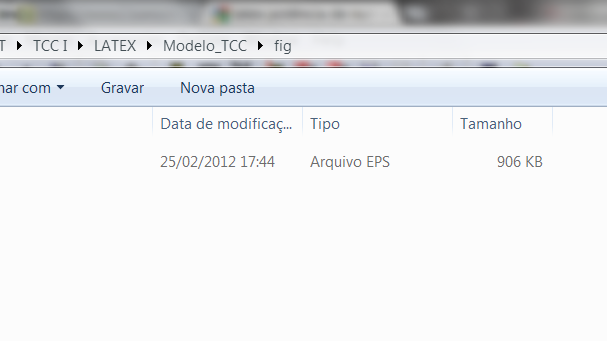
\includegraphics[width=10cm]{fig/estruturaneuronio}
    \label{estruturaneuronio}
    \caption{Estrutura de um neur�nio}
\end{figure}

\section{Teoria da Sele��o de Grupos Neuronais}



\section{Modelos de Neur�nios}

\section{Modelo de Sinapse}

\section{Codifica��o neural}

\section{Detec��o de coincid�ncias}

\section{Considera��es Finais} 
  %    Trabalho de Conclus�o de Curso
%
% Centro Federal de Educa��o Tecnol�gica de Minas Gerais - CEFET-MG
% Autor: Thaiana Hofman do Bom Conselho
%
% Parte: Modelagem e Desenvolvimento Sistemas Neurais

\chapter{Modelagem e Desenvolvimento Sistemas Neurais}\label{modelagem}

\section{Introdu��o}

\section{Modelos computacionais biologicamente plaus�veis}

\section{Neur�nios Pulsantes}

\section{Modelo de neur�nio pulsante de Izhikevich}

\section{Sinapses}

\section{Spike-timing-dependent plasticity}

\section{Considera��es Finais}

  %    Trabalho de Conclus�o de Curso
%
% Centro Federal de Educa��o Tecnol�gica de Minas Gerais - CEFET-MG
% Autor: Thaiana Hofman do Bom Conselho
%
% Parte: Rob�s Aut�nomos Bioinspirados

\chapter{Rob�s Aut�nomos Bioinspirados}\label{robosAuto}

\section{Introdu��o}

\section{Rob�s Aut�nomos}

\section{Considera��es Finais}

  %    Trabalho de Conclus�o de Curso
%
% Centro Federal de Educa��o Tecnol�gica de Minas Gerais - CEFET-MG
% Autor: Thaiana Hofman do Bom Conselho
%
% Parte: Experimentos Computacionais

\chapter{Experimentos Computacionais}\label{experimentos}

\section{Introdu��o}

\section{Detector de Coincid�ncias}

\section{Circuito Sens�rio-Motoro}

\section{RoboDeck}

\section{Curumim}

\section{Apresenta��o dos Resultados e Experimentos}

\section{Considera��es Finais}

  %    Trabalho de Conclus�o de Curso
%
% Centro Federal de Educa��o Tecnol�gica de Minas Gerais - CEFET-MG
% Autor: Thaiana Hofman do Bom Conselho
%
% Parte: Conclus�o

\chapter{Conclus�o}\label{conclusao}

\section{Discuss�o do Trabalho}

\section{Trabalhos Futuros}

  
  %
% Documento: Referências Bibliográficas
%

\bibliographystyle{abnt-alf}
\bibliography{./bibliografia}	% geracao automatica das referencias a partir do arquivo refbase.bib

%  %	 Modelo de Projeto de disserta��o de mestrado
%
% Centro Federal de Educa��o Tecnol�gica de Minas Gerais - CEFET-MG
% Departamento de Pesquisa e P�s-Gradua��o - DPPG
% Autor: Grupo de Pesquisas em Sistemas Inteligentes (GPSI)
%
% Parte: Anexos

\apendice

\chapter{T�TULO DO AP�NDICE}

Incluir os ap�ndices ao corpo principal do projeto de disserta��o.

\ProximoForaDoSumario\section{Poderia ser uma se��o (Mas n�o aparece no sum�rio)}
Um par�grafo.

\ProximoForaDoSumario\section{Esta seria outra se��o (Mas n�o aparece  sum�rio)}
Um par�grafo.

\chapter{T�TULO DO AP�NDICE}

Este � outro ap�ndice.

\ProximoForaDoSumario\section{Uma se��o do ap�ndice B (N�o aparece no sum�rio)}
Um par�grafo.
%  %	 Modelo de Projeto de disserta��o de mestrado
%
% Centro Federal de Educa��o Tecnol�gica de Minas Gerais - CEFET-MG
% Departamento de Pesquisa e P�s-Gradua��o - DPPG
% Autor: Grupo de Pesquisas em Sistemas Inteligentes (GPSI)
%
% Parte: Anexos

\anexo

\chapter{T�TULO DO ANEXO}

Incluir os anexos ao corpo principal do projeto de disserta��o.

Pode ser que seja necess�rio divid�-lo em se��es e subse��es. Neste caso use o mesmo esquema descrito nos demais cap�tulos deste documento modelo.

\ProximoForaDoSumario\section{Poderia ser uma se��o (Mas n�o aparece no sum�rio)}
Um par�grafo.

\ProximoForaDoSumario\section{Esta seria outra se��o (Mas n�o aparece  sum�rio)}
Um par�grafo.

\chapter{T�TULO DO ANEXO}

Este � outro anexo. Se for necess�rio divid�-lo em se��es e sub--se��es, proceda como relatado no Anexo A deste documento modelo.

\ProximoForaDoSumario\section{Uma se��o do anexo B (N�o aparece no sum�rio)}
Um par�grafo.
%  %	 Modelo de Projeto de disserta��o de mestrado
%
% Centro Federal de Educa��o Tecnol�gica de Minas Gerais - CEFET-MG
% Departamento de Pesquisa e P�s-Gradua��o - DPPG
% Autor: Grupo de Pesquisas em Sistemas Inteligentes (GPSI)
%
% Parte: �ndice Remissivo

\chapter*{�ndices}
A seguir s�o apresentados �ndices remissivos (cita��es e alfab�tico) com o intuito de facilitar a localiza��o de informa��es no documento.
\ProximoForaDoSumario\printindex{citacao}{\textit{�ndice Remissivo (Cita��es)}}
\ProximoForaDoSumario\printindex{alfa}{\textit{�ndice Remissivo (Alfab�tico)}}


\end{document}
